\let\negmedspace\undefined
\let\negthickspace\undefined
\documentclass[journal]{IEEEtran}
\usepackage[a5paper, margin=10mm, onecolumn]{geometry}
\usepackage{lmodern} % Ensure lmodern is loaded for pdflatex
\usepackage{tfrupee} % Include tfrupee package

\setlength{\headheight}{1cm} % Set the height of the header box
\setlength{\headsep}{0mm}     % Set the distance between the header box and the top of the text

\usepackage{gvv-book}
\usepackage{gvv}
\usepackage{cite}
\usepackage{amsmath,amssymb,amsfonts,amsthm}
\usepackage{algorithmic}
\usepackage{graphicx}
\usepackage{textcomp}
\usepackage{xcolor}
\usepackage{txfonts}
\usepackage{listings}
\usepackage{enumitem}
\usepackage{mathtools}
\usepackage{gensymb}
\usepackage{comment}
\usepackage[breaklinks=true]{hyperref}
\usepackage{tkz-euclide} 
\usepackage{listings}
\def\inputGnumericTable{}                                 
\usepackage[latin1]{inputenc}                                
\usepackage{color}                                            
\usepackage{array}                                            
\usepackage{longtable}                                       
\usepackage{calc}                                             
\usepackage{multirow}                                         
\usepackage{hhline}                                           
\usepackage{ifthen}                                           
\usepackage{lscape}

\begin{document}

\bibliographystyle{IEEEtran}
\vspace{3cm}

\title{6.5.13}
\author{EE24BTECH11036 - Krishna Patil}
% \maketitle
% \newpage
% \bigskip
{\let\newpage\relax\maketitle}

\renewcommand{\thefigure}{\theenumi}
\renewcommand{\thetable}{\theenumi}
\setlength{\intextsep}{10pt} % Space between text and floats

\renewcommand{\thefigure}{\theenumi}
\renewcommand{\thetable}{\theenumi}
\setlength{\intextsep}{10pt} % Space between text and floats

\textbf{Question :}  Find two numbers whose sum is 24 and whose product is as large as possible. \\

\solution \\

Let the two numbers be $ x $ and $ y $. We are given the following conditions:

\begin{enumerate}
    \item The sum of the numbers is 24:
    \begin{align}
        x + y = 24
    \end{align}
    \item We need to maximize the product $ P = x \cdot y $.
\end{enumerate}

\textbf{Express $ y $ in terms of $ x $}  
From the equation $ x + y = 24 $, we can solve for $ y $:
\begin{align}
    y = 24 - x
\end{align}

\textbf{Write the product in terms of $ x $}  
Substitute $ y = 24 - x $ into the product equation:
\begin{align}
    P\brak{x} = x \cdot \brak{24 - x} = 24x - x^2
\end{align}
We want to maximize this quadratic expression for $ P\brak{x} $.

\textbf{Find the value of $ x $ that maximizes $ P\brak{x} $}  
To maximize $ P\brak{x} = 24x - x^2 $, we first take the derivative of $ P\brak{x} $ with respect to $ x $:
\begin{align}
    P{^\prime}\brak{x} = 24 - 2x
\end{align}
Next, we set the derivative equal to zero to find the critical points:
\begin{align}
    24 - 2x = 0
\end{align}
Solving for $ x $:
\begin{align}
    2x = 24 \implies x = 12
\end{align}

\textbf{Verify that this is a maximum}  
To ensure that $ x = 12 $ gives a maximum, we take the second derivative of $ P\brak{x} $:
\begin{align}
    P{^\prime}{^\prime}\brak{x} = -2
\end{align}
Since $ P{^\prime}{^\prime}\brak{x} = -2 $ is negative, the function $ P\brak{x} $ is concave down, confirming that $ x = 12 $ is indeed a maximum.

\textbf{Find the value of $ y $}  
Since $ x = 12 $, substitute this into the equation $ y = 24 - x $ :
\begin{align}
    y = 24 - 12 = 12
\end{align}

\textbf{Calculate the maximum product}  
Now, we calculate the product of the two numbers:
\begin{align}
    P = 12 \cdot 12 = 144
\end{align}

\textbf{Conclusion:} The two numbers are 12 and 12, and their product is 144. Therefore, the maximum product of two numbers whose sum is 24 is 144. \\

\textbf{Gradient Descent Algorithm}:
We use the method of gradient descent to find the maximum of the given function, since the objective function is convex.
Since the coefficient of $\brak{24x-x^2} < 0$, we expect to find the maximum.
\begin{align}
    x_{n+1} &= x_n - \mu f^{\prime}\brak{x_n}\\
    f^{\prime}\brak{x_n} &= 24 - 2x_n\\
    \xrightarrow{} x_{n+1} &= x_n - \mu\brak{24 - 2x_n} \\
    &= \brak{1+2\mu}x_n -24\mu
\end{align}
Applying unilateral Z-transform,
1. Apply $ Z[\lambda_n] = Y\brak{z} $:
   \begin{align}
   zY(z) - z\lambda_0 = \brak{1+2\mu}Y(z) - 24\mu \frac{z}{z-1}
   \end{align}
2. Rearrange:
   \begin{align}
   Y(z)(z - \brak{1+2\mu}) = z\lambda_0 - 24\mu \frac{z}{z-1}
   \end{align}
3. Solve for $ Y\brak{z} $:
   \begin{align}
   Y(z) = \frac{\lambda_0 z}{z-\brak{1+2\mu}} - \frac{24\mu z}{(z-1)(z-\brak{1+2\mu})}
   \end{align}

Take the inverse $ Z $-transform:
\begin{align}
\lambda_n &= \brak{1+2\mu}^n \lambda_0 + 1 - \brak{24\mu +12}\brak{1+2\mu}^{n-1} \\
\lambda_n &= \brak{1+2\mu}^n \lambda_0 + 12 - 12\brak{1+2\mu}^n
\end{align}

But say initial guess , $\lambda_0 = 0 $ so,
\begin{align}
\lambda_n &=  12\brak{1 - \brak{1+2\mu}^n}
\end{align}

For Radius of convergence , using ratio test , we get ,
\begin{align}
\mu < 0 
\end{align}

Taking initial guess = 0 , step size = 0.01 ,tolerance(minimum value of gradient) = 1e-5 , We get 
$x_{min} \approx 12 $. \\

\textbf{Geometric Programming} :

We generally use geometric programming for minimize so instead of maximizing $24x - x^2$,we minimize $x^2 -24x$.
We solve it using $cvxpy$ module in python. On running the code we, get maximum value at $x$ is, $12.00000$, so, maximum product value is $144.00000$.

\begin{figure}[h!]
   \centering
   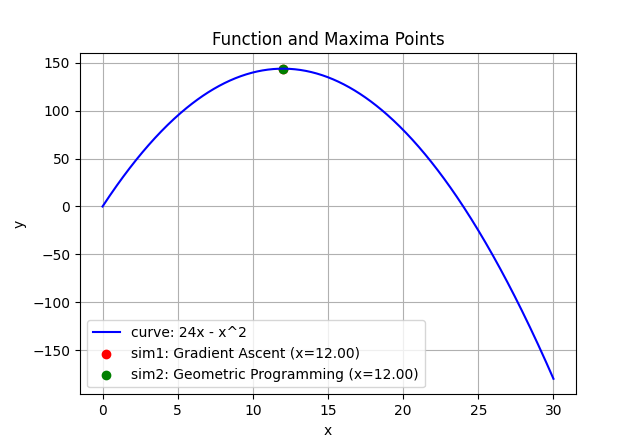
\includegraphics[width=0.7\linewidth]{figs/Figure_1.png}
\end{figure}
\end{document}

